\documentclass{standalone}
\usepackage{tikz}
\usetikzlibrary{automata,positioning}
\begin{document}
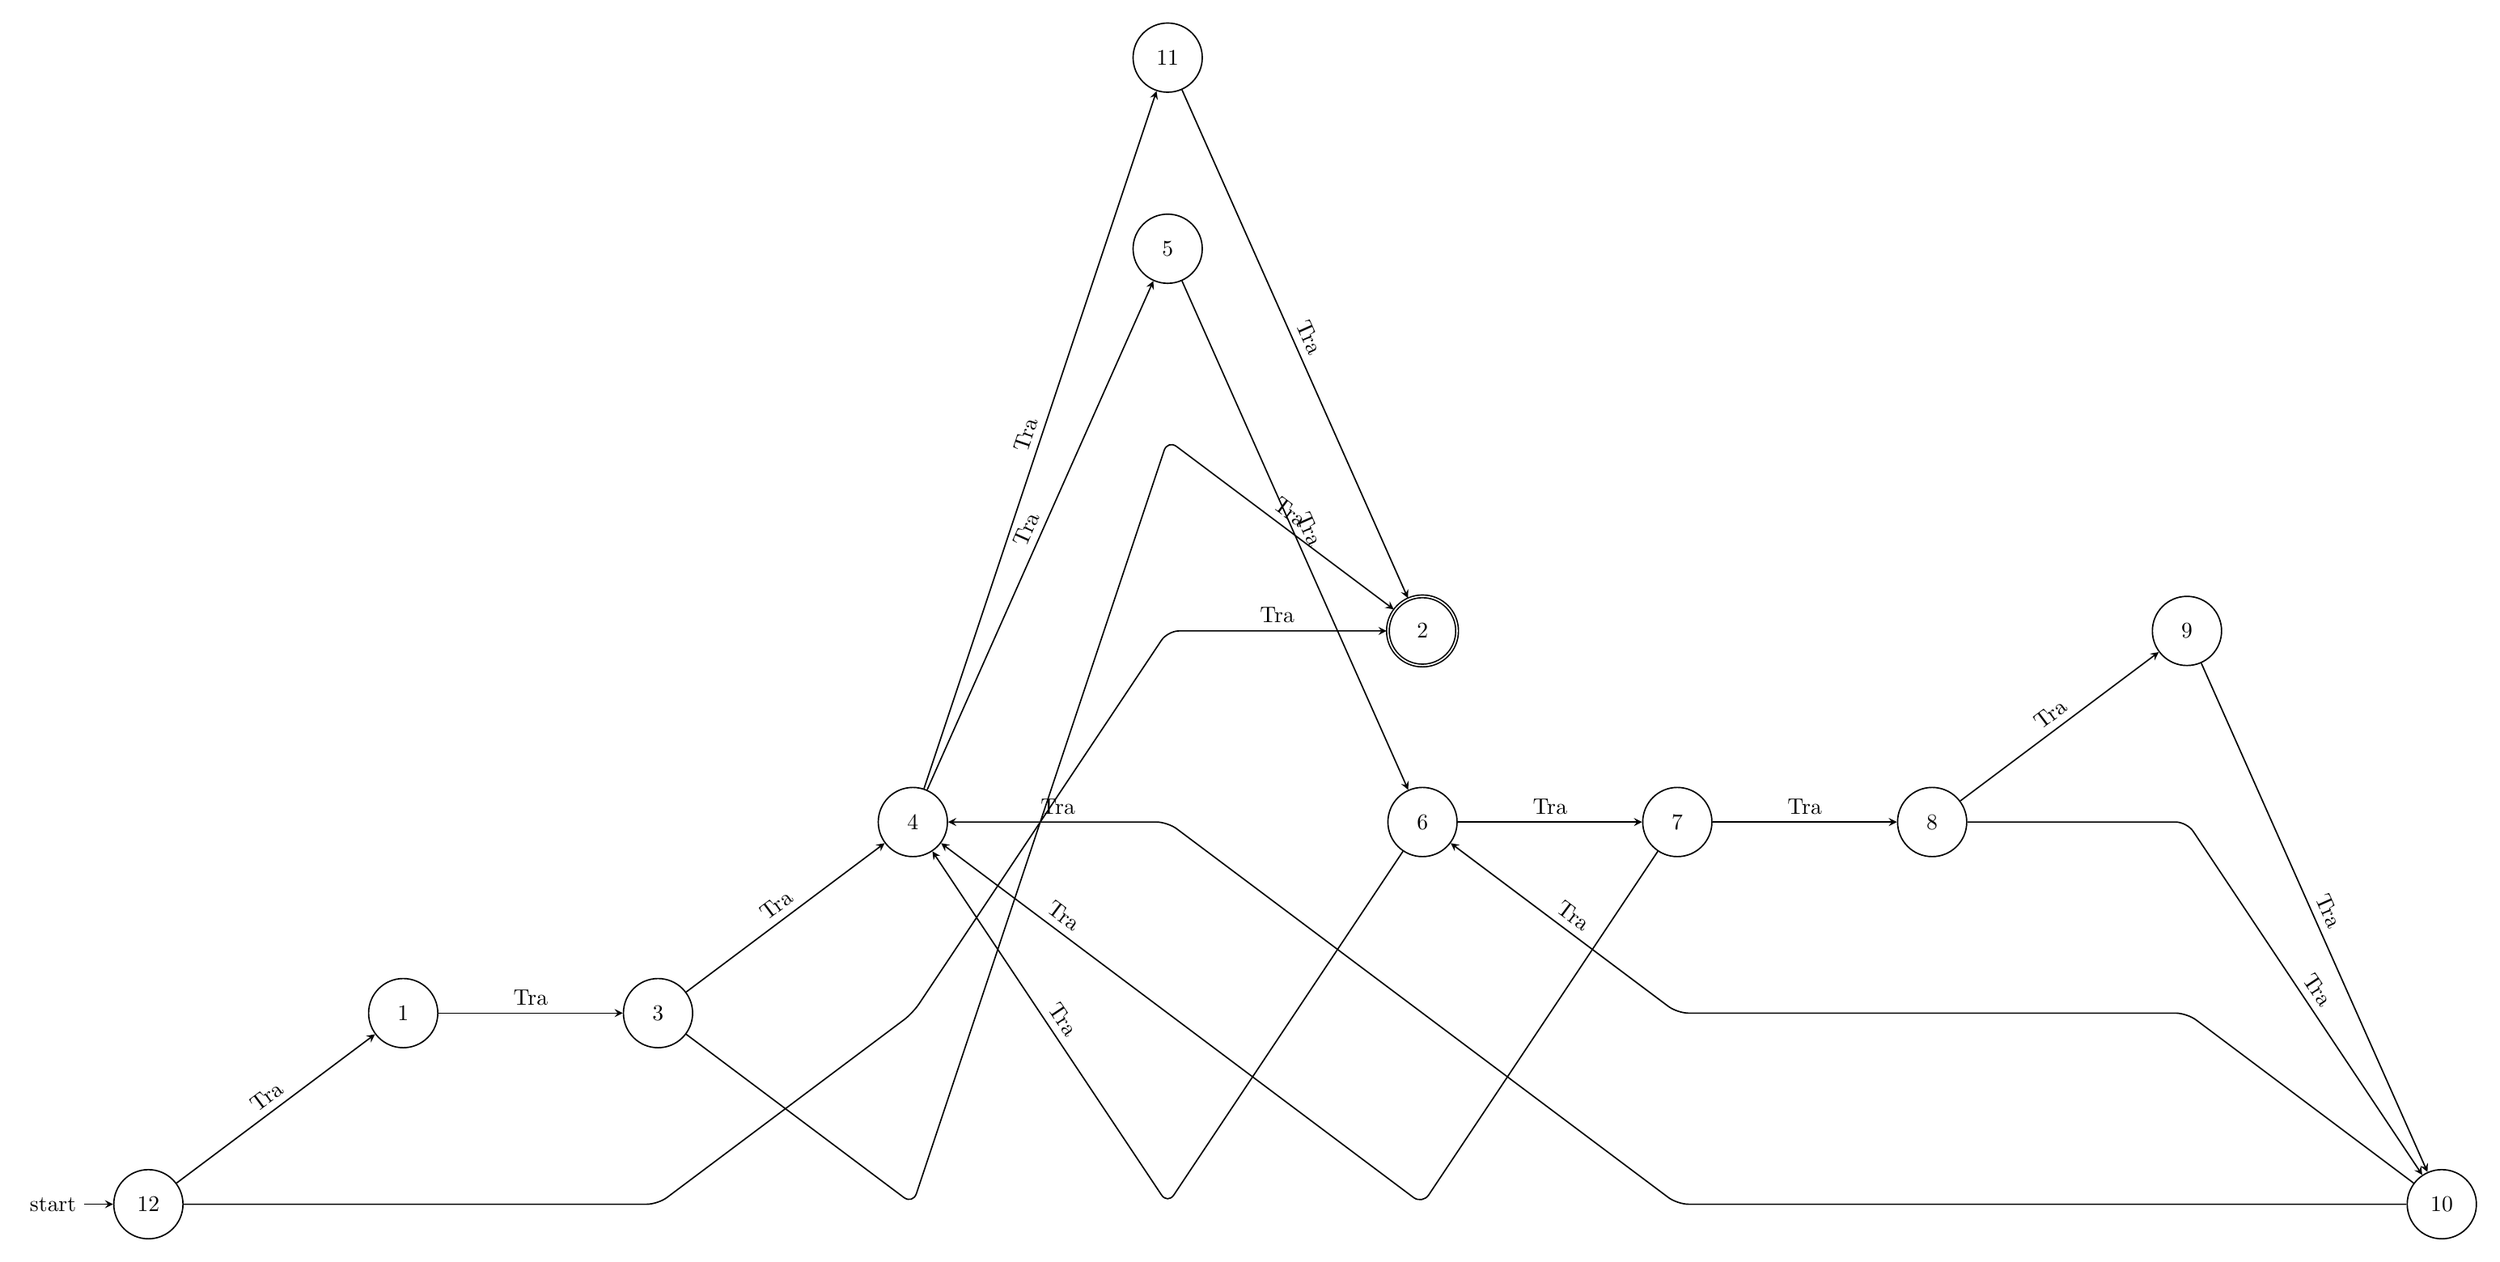
\begin{tikzpicture}[->,>=stealth,auto,node distance=2.5cm,semithick,every state/.style={minimum width=1cm, minimum height=1cm, text width=0.75cm,align=center}]
\node[state, initial] (12) at (0,0) {12};
\node[state] (1) at (4,3) {1};
\node[state, accepting] (2) at (20,9) {2};
\node[state] (3) at (8,3) {3};
\node[state] (4) at (12,6) {4};
\node[state] (5) at (16,15) {5};
\node[state] (6) at (20,6) {6};
\node[state] (7) at (24,6) {7};
\node[state] (8) at (28,6) {8};
\node[state] (9) at (32,9) {9};
\node[state] (10) at (36,0) {10};
\node[state] (11) at (16,18) {11};
\draw[->, rounded corners=5pt] (12) -- (4,0) -- (8,0) -- (12,3) -- (16,9) -- (2) node[midway, sloped, above] {Tra};
\draw[->, rounded corners=5pt] (3) -- (12,0) -- (16,12) -- (2) node[midway, sloped, above] {Tra};
\draw[->, rounded corners=5pt] (6) -- (16,0) -- (4) node[midway, sloped, above] {Tra};
\draw[->, rounded corners=5pt] (7) -- (20,0) -- (16,3) -- (4) node[midway, sloped, above] {Tra};
\draw[->, rounded corners=5pt] (8) -- (32,6) -- (10) node[midway, sloped, above] {Tra};
\draw[->, rounded corners=5pt] (10) -- (32,0) -- (28,0) -- (24,0) -- (20,3) -- (16,6) -- (4) node[midway, sloped, above] {Tra};
\draw[->, rounded corners=5pt] (10) -- (32,3) -- (28,3) -- (24,3) -- (6) node[midway, sloped, above] {Tra};
\path (12) edge node[midway, sloped, above] {Tra} (1);
\path (1) edge node[midway, sloped, above] {Tra} (3);
\path (3) edge node[midway, sloped, above] {Tra} (4);
\path (4) edge node[midway, sloped, above] {Tra} (5);
\path (5) edge node[midway, sloped, above] {Tra} (6);
\path (6) edge node[midway, sloped, above] {Tra} (7);
\path (7) edge node[midway, sloped, above] {Tra} (8);
\path (8) edge node[midway, sloped, above] {Tra} (9);
\path (9) edge node[midway, sloped, above] {Tra} (10);
\path (4) edge node[midway, sloped, above] {Tra} (11);
\path (11) edge node[midway, sloped, above] {Tra} (2);
\end{tikzpicture}
\end{document}